\section{Skeletons}
\label{sec:skeletons}
Now we have developed Parallel Arrows far enough to define some useful algorithmic skeletons that abstract typical parallel computations. While there are many possible skeletons to implement, we regard in detail here only some |map|-based and topological skeletons to demonstrate the power of PArrows.
%%% \FloatBarrier
\subsection{|map|-based Skeletons}
\label{sec:map-skeletons}
We start with |map|-based skeletons. The essential differences between the skeletons presented here are in terms of order of evaluation and work distribution but still provide the same output of a standard |map|. 

\paragraph{Parallel |map| and laziness.}
The |parMap| skeleton (Figs.~\ref{fig:parMapImg},~\ref{fig:parMap}) is probably the most common skeleton for parallel programs. We can implement it with |ArrowParallel| by repeating an arrow |arr a b| and then passing it into |parEvalN| to obtain an arrow |arr [a] [b]|.
Just like |parEvalN|, |parMap| is 100\% strict.
Because of this, it has the same restrictions as |parEvalN| as compared to |parEvalNLazy|. So it makes sense to also have a |parMapStream| (Figs.~\ref{fig:parMapStreamImg},~\ref{fig:parMapStream}) which behaves like |parMap|, but uses |parEvalNLazy| instead of |parEvalN|. The code of these two skeletons is quite straightforward, we show it in Appendix.

\begin{figure}[thb]
%farm
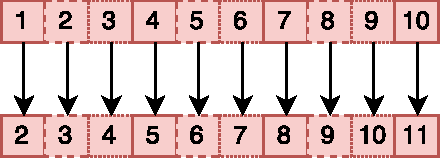
\includegraphics[scale=0.7]{images/farm}
\caption{Schematic depiction of a |farm|, a statically
      load-balanced |parMap|.}
\label{fig:farmImg}

\begin{code}
farm :: (ArrowParallel arr a b conf,
	ArrowParallel arr [a] [b] conf, ArrowChoice arr) =>
	conf -> NumCores -> arr a b -> arr [a] [b]
farm conf numCores f =
	unshuffle numCores >>>
	parEvalN conf (repeat (mapArr f)) >>>
	shuffle
\end{code}
\caption{The definition of |farm|.}
\label{fig:farm}

%farmChunk
\includegraphics[scale=0.7]{images/farmChunk}
\caption{Schematic depiction of |farmChunk|.}
\label{fig:farmChunkImg}
\end{figure}

\paragraph{Statically load-balancing parallel |map|.}
Our |parMap| spawns every single computation in a new thread (at least for the instances of |ArrowParallel| we gave in this paper). This can be quite wasteful and a statically load-balancing |farm| (Figs.~\ref{fig:farmImg},~\ref{fig:farm}) that equally distributes the workload over |numCores| workers seems useful.
The definitions of the helper functions |unshuffle|, |takeEach|, |shuffle| (Fig.~\ref{fig:edenshuffleetc}) originate from an Eden skeleton\footnote{Available on Hackage under \url{https://hackage.haskell.org/package/edenskel-2.1.0.0/docs/src/Control-Parallel-Eden-Map.html}.}.

%\paragraph{Lazy statically load-balancing parallel map}
Since a |farm|  is basically just |parMap| with a different work distribution, it is, again, 100\% strict. So we can define |farmChunk| (Figs.~\ref{fig:farmChunkImg},~\ref{fig:farmChunk}) which uses |parEvalNLazy| instead of |parEvalN|. It is basically the same definition as for |farm|, with |parEvalN| replaced with |parEvalNLazy|.

%%% Local Variables:
%%% mode: latex
%%% TeX-master: "main"
%%% End:
